\documentclass{tccv}
\usepackage[english]{babel}
\usepackage[utf8]{inputenc}							% For easy input with é 
\usepackage[T1]{fontenc}							% For true french font 
\usepackage{lmodern}								% For scalable font in T1 (instead of OT1).
\usepackage{amsfonts} 								% for the \checkmark command 
\usepackage[pdftex]{graphicx}							% Enable pdflatex and includegraphics = foto pona
\usepackage{vwcol} 								% Avoir des colu,ne de tailles differerentes
\usepackage[framemethod=TikZ]{mdframed}

 \usepackage[hmargin=0.2cm,vmargin=0cm]{geometry}

\usepackage[overlay,absolute]{textpos}
\setlength{\TPHorizModule}{1cm}
\setlength{\TPVertModule}{1cm}



\mdfsetup{%
   middlelinecolor=blue,
   middlelinewidth=2pt,
   backgroundcolor=white!0,
   roundcorner=10pt,
   skipabove=0,   
   fontcolor=black,
   }


\begin{document}
%%%%%%%%%%%%%%%%%%%%%%%%%%%%%%%%%%%%%%%%%%%%%%%%%%%%%%%%%%%%%%%%%%%%%%%%%%%%%%%%%%%%%%%%%%%%%%%%%%%%%%%%%%%%%%%%%%%%


\begin{textblock}{6.5}(0.5,0.5)
\personal
    []
    {16 Rue Chicogné, 35000 -- Rennes}
    {+33 07 83 88 33 32}
    {r.sanhuezarepetto@gmail.com}
\end{textblock}

\begin{textblock}{10}(8.5,1)
    \usekomafont{part} Roc\'io Sanhueza
\end{textblock}

\begin{textblock}{21}(17.5,0.5)
		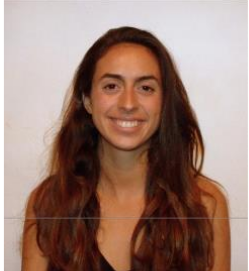
\includegraphics[width=3cm]{../Figure/Rocio1.png}
\end{textblock}  









\begin{textblock}{7}(0.2,4)
\begin{mdframed}

\section{Education}
\begin{yearlist}

\item[Master 1 Science politique]{2015 -- 2016}
     {Université de Rennes 1}
     {Enseignements suivis: pensée politique contemporaine, 
     régimes contemporaines, sociologie de la communication, pensée sociologique, Approches de l'Union Européen, Grand dossiers de l'administration.}


  

\item[Diplôme en Communication sociale et journalisme]{2008 -- 2013}
     {Universidad de Santiago de Chile}
     {Mention très bien
      Spécialité politique
      (Bac+5)}

     
\item[Échange universitaire -- journalisme]{2011 -- 2011}
     {Universidade Estadual Paulista (UNESP)}
     {Enseignements suivis: réalité socio-économique et politique brésilienne, langue portugaise: littérature, sémiotique, stratégies de communication publique}


\end{yearlist}
\end{mdframed}


\begin{mdframed}
\section{Compétences linguistiques}

\begin{factlist}
\item{Espagnol} {Langue maternelle}	
\item{Français} {Courant}	
\item{Anglais}  {Niveau B2}	
\item{Portugais}{Niveau B2}
\end{factlist}

\section{Logiciels}

Environnement PC et Linux,
Pack office et libre office,
Adobe Photoshop, Premiere, \\
 \\
%Python, 
Gimp,
HTML5,
\LaTeX.

%%%%%%%%%%%%%%%%%%%%%%%%%%%%%%%%%%%%%%%%%%%%%%%%%%%%%%%%%%%%%%%%%%%%%%%%%%%%%%%%%%%%%%%%%%%%%%%%%%%%%%%%%%%%%%%%%%%%%%%%%%%%%%%%%%%%%%%%%%
%&
\end{mdframed}
\end{textblock}


\mdfsetup{middlelinecolor=white!0}

\begin{textblock}{13}(7.7,4)
\begin{mdframed}
\section{Experience Professionnelle}


\begin{eventlist}
\item{Avril 2014 -- Mars 2015}
     {Sénat du Chili, Santiago, Chili}
     {Conseillère en communication et attachée de presse}

     
     % Missions
    \begin{itemize}
      \setlength\itemsep{0cm} 
      \cvitem[\checkmark] Chargée de la mise en œuvre des actions de communication et des relations avec la presse nationale et régionale
      \cvitem[\checkmark] Rédaction des articles, communiqués et dossiers de presse. Gestion et supervision des interviews avec des chaînes de télévision
      \cvitem[\checkmark] Organisation des conférences de presse
      \cvitem[\checkmark] Administration de réseaux sociaux conjointement avec l’administrateur du site web
    \end{itemize}     
     


\item{Mai 2013 -- Déc. 2014}
     {Aluro 35, Santiago, Chili}
     {Productrice générale}
    
    \begin{itemize}
      \setlength\itemsep{0cm} 
      \cvitem[\checkmark] Gérer les rapports avec la chaîne de télévision et négociation avec eux les budgets. Recherche des marques sponsors
      \cvitem[\checkmark] Préparation du lieu de tournage, mobilisation, catering et interviewés de chaque chapitre. Aide à la préparation du contenu des entretiens
      \cvitem[\checkmark] Administration de réseaux sociaux et animation de communautés (Facebook, Twitter, Instagram)
      \cvitem[\checkmark] Création du dossier de presse pour les lancements des deux premières sessions du programme

    \end{itemize}     

\item{Oct. 2013 -- Fév. 2014 }     
  {Agence de communication Más comunicaciones, Santiago, Chili}     
  {Journaliste}

\begin{itemize}
      \setlength\itemsep{0cm} 
      \cvitem[\checkmark] Préparation des articles pour les médias
      \cvitem[\checkmark] Création des dossiers de presse 
      \cvitem[\checkmark] Cibler les journalistes spécialisés et améliorer régulièrement la basse de donnés. 
      \cvitem[\checkmark] Relances téléphoniques
\end{itemize}       



\item{Avril 2012 -- Avril 2013 }     
  {Killahue corporation, Santiago, Chili}     
  {Chargée de projet}

\begin{itemize}
      \setlength\itemsep{0cm} 
      \cvitem[\checkmark] Recherche des informations juridiques et environnementales des projets similaires dans le cadre national ou internationale
      \cvitem[\checkmark] Gestion et coordination des réunions chaque semaine avec les membres de la corporation, plus la préparation des matériaux visuel et écrit
      \cvitem[\checkmark] Administration de réseaux sociaux 
      \cvitem[\checkmark] Formalisation et rédaction du travail réalisé et des décisions pris dans l’ensemble des réunions

\end{itemize}      
    
\iffalse
\item{Janv. 2012 -- Mars 2012 }     
  {Terra Networks, Santiago, Chili}     
  {Journaliste stagiaire – section économie}

\begin{itemize}
      \setlength\itemsep{0cm} 
      \cvitem[\checkmark] Rédaction des articles et notes d’économie national et internationale
      \cvitem[\checkmark] Traduction des nouvelles du portugais ou anglaise au espagnol
      \cvitem[\checkmark] Veille et mise à jour du site économique
      \cvitem[\checkmark] Réalisation des interviews et couverture médiatique des thèmes économiques nationaux

\end{itemize}        
\fi
   


\end{eventlist}


\end{mdframed}
\end{textblock}
\end{document}
